

\documentclass[
  size=14pt,
  paper=smartboard,  %a4paper, smartboard, screen
  mode=present, 		%present, handout, print
  display=slides, 	% slidesnotes, notes, slides
  style=tuliplab,  	% TULIP Lab style
  pauseslide,
  fleqn,leqno]{powerdot}
 
\usepackage{hyperref}
\usepackage{graphicx}
 \usepackage{amssymb}
 \usepackage{amsmath}
 \usepackage{rotating}
 \usepackage{graphicx}
 \usepackage{boxedminipage}
 \usepackage{media9}
 \usepackage{rotate}
 \usepackage{calc}
 \usepackage[absolute]{textpos}
 \usepackage{psfrag,overpic}
 \usepackage{fouriernc}
 \usepackage{pstricks,pst-node,pst-text,pst-3d,pst-grad}
 \usepackage{moreverb,epsfig,subfigure}
 \usepackage{pstricks}
 \usepackage{pstricks-add}
 \usepackage{pst-text}
 \usepackage{pst-node, pst-tree}
 \usepackage{booktabs}
 \usepackage{etex}
 \usepackage{breqn}
 \usepackage{multirow}
 \usepackage{gitinfo2}
 \usepackage{xcolor}
 \usepackage{epsfig}
 
 \usepackage{todonotes}
 % \usepackage{pst-rel-points}
 \usepackage{animate}
 \usepackage{fontawesome}
 
 \usepackage{listings}
 \lstset{frameround=fttt,
 frame=trBL,
 stringstyle=\ttfamily,
 backgroundcolor=\color{yellow!20},
 basicstyle=\footnotesize\ttfamily}
 \lstnewenvironment{code}{
 \lstset{frame=single,escapeinside=`',
 backgroundcolor=\color{yellow!20},
 basicstyle=\footnotesize\ttfamily}
 }{}
 
 \usepackage{hyperref}
 \hypersetup{ % TODO: PDF meta Data
   pdftitle={Presentation Title},
   pdfauthor={Gang Li},
   pdfpagemode={FullScreen},
   pdfborder={0 0 0}
 }
 
 % \usepackage{auto-pst-pdf}
 % package to show source code
 
 \definecolor{LightGray}{rgb}{0.9,0.9,0.9}
 \newlength{\pixel}\setlength\pixel{0.000714285714\slidewidth}
 \setlength{\TPHorizModule}{\slidewidth}
 \setlength{\TPVertModule}{\slideheight}
 \newcommand\highlight[1]{\fbox{#1}}
 \newcommand\icite[1]{{\footnotesize [#1]}}
 
 \newcommand\twotonebox[2]{\fcolorbox{pdcolor2}{pdcolor2}
 {#1\vphantom{#2}}\fcolorbox{pdcolor2}{white}{#2\vphantom{#1}}}
 \newcommand\twotoneboxo[2]{\fcolorbox{pdcolor2}{pdcolor2}
 {#1}\fcolorbox{pdcolor2}{white}{#2}}
 \newcommand\vpspace[1]{\vphantom{\vspace{#1}}}
 \newcommand\hpspace[1]{\hphantom{\hspace{#1}}}
 \newcommand\COMMENT[1]{}
 
 \newcommand\placepos[3]{\hbox to\z@{\kern#1
         \raisebox{-#2}[\z@][\z@]{#3}\hss}\ignorespaces}
 
 \renewcommand{\baselinestretch}{1.2}
 
 
 \newcommand{\draftnote}[3]{
   \todo[author=#2,color=#1!30,size=\footnotesize]{\textsf{#3}}	}
 % TODO: add yourself here:
 %
 \newcommand{\gangli}[1]{\draftnote{blue}{GLi:}{#1}}
 \newcommand{\shaoni}[1]{\draftnote{green}{sn:}{#1}}
 \newcommand{\gliMarker}
   {\todo[author=GLi,size=\tiny,inline,color=blue!40]
   {Gang Li has worked up to here.}}
 \newcommand{\snMarker}
   {\todo[author=Sn,size=\tiny,inline,color=green!40]
   {Shaoni has worked up to here.}}

%%%%%%%%%%%%%%%%%%%%%%%%%%%%%%%%%%%%%%%%%%%%%%%%%%%%%%%%%%%%%%%%%%%%%%%%
% title
% TODO: Customize to your Own Title, Name, Address
%
\title{Flip00 Presentation}
\author{
Tao Yu
\\
\\Xi'an Shiyou University
}
% \date{September 2020}
\date{\gitCommitterDate}

% Customize the setting of slides
% \pdsetup{
% TODO: Customize the left footer, and right footer
% rf=\href{http://www.tulip.org.au}{
% Last Changed by: (\gitAuthorDate)
% },
% cf={Flip00 Presentation},
% }

\pdsetup{
% TODO: Customize the left footer, and right footer
rf=\href{http://www.tulip.org.au}{
Last Changed by: \textsc{\gitCommitterName}\ \gitVtagn-\gitAbbrevHash\ (\gitAuthorDate)
},
cf={Group Outlying Aspects Mining},
}

\begin{document}

\maketitle

%\begin{slide}{Overview}
%\tableofcontents[content=sections]
%\end{slide}


%%==========================================================================================
%%
\begin{slide}[toc=,bm=]{Content}
\tableofcontents[content=currentsection,type=1]
\end{slide}
%%
%%==========================================================================================


%\section{Problem Definition}


%%==========================================================================================
%%
%------留下
\section{Introduction}
\begin{slide}{Introduction}
\begin{center}
\twotonebox{\rotatebox{90}{Defn}}{\parbox{.86\textwidth}
{Introduction to \textcolor{orange}{Bike Sharing }Project.
\begin{itemize}
\item 
The influence of weather, time, humidity, wind speed, seasons, holidays and other factors on bicycle usage.
\\
\item 
Analyze and predict bicycle usage.\\
\end{itemize}
}}
\end{center}
\bigskip
\begin{center}

\end{center}
\bigskip
\end{slide}

% \begin{slide}{Introduction}
%   %Challenges (1)
%   \begin{itemize}
%   \item
%   Introduction to \textcolor{orange}{Bike Sharing }Project.
%   \begin{itemize}
%   \item
%   The influence of weather, time, humidity, wind speed, seasons, holidays and other factors on bicycle usage.
%   \item
%   Analyze and predict bicycle usage.\\
%   \end{itemize}
%   \end{itemize}
%   \end{slide}

\section{Data analysis and processing}
  \begin{slide}{Data analysis}
    %Challenges (1)
    \begin{tabular}{c| c c c c c c c c }
    \toprule
    Data & \texttt{season}  & \texttt{holiday}  & \texttt{weather}    & \texttt{humidity} & \texttt{windspeed} & \texttt{registered} & \texttt{count}\\
    \midrule
    $count$
    &  {$10886.00$} &  {$10886.00$} &  {$10886.00$} &  {$10886.00$} &  {$10886.00$} & {$10886.00$} & {$10886.00$}\\
    $mean$
    &  {$2.506614$} &  {$0.028569$}&  {$1.418427$}&  {$61.886460$} &  {$12.799395$}&  {$155.552177$}&  {$191.574132$}\\
    $std$
    &  {$1.116174$} &  {$0.166599$} &  {$0.633839$} &  {$19.245033$} &  {$8.164537$}&  {$151.039033$}&  {$181.144454$}& \\
    $min$
    &  {$1.000000$} &  {$0.000000$}&  {$1.000000$}&  {$0.000000$} &  {$0.000000$}&  {$0.000000$}&  {$1.000000$}\\
    ${25\%}$
    &  {$2.000000$} &  {$0.000000$} &  {$1.000000$} &  {$47.000000$}&  {$7.001500$} &  {$36.000000$} &  {$42.000000$}\\
    ${50\%}$
    &  {$3.000000$} &  {$0.000000$} &  {$1.000000$} &  {$62.000000$}&  {$12.998000$} &  {$118.000000$} &  {$145.000000$}\\
    ${75\%}$
    &  {$4.000000$} &  {$0.000000$} &  {$2.000000$} &  {$77.000000$}&  {$16.997900$} &  {$222.000000$} &  {$284.000000$}\\
    $max$
    &  {$4.000000$} &  {$1.000000$} &  {$4.000000$} &  {$100.000000$}&  {$56.996900$} &  {$886.000000$} &  {$977.0000$}\\
    \bottomrule
    \end{tabular}
    \\
      \begin{itemize}
      \item
      From the figure, the standard deviation of the rental volume we need to forecast is very large.
      \item
      So let's look at the distribution.\\
      \end{itemize}
    \end{slide}

    \begin{slide}{Data processing 1}
      %Challenges (1)
      \begin{itemize}
      \item
      The whole distribution inclines seriously and needs to be dealt with in order to avoid over fitting in the end.
      \end{itemize}
        \begin{figure}[htb]
          \centering
          %\missingfigure[figwidth=16cm]{Testing a long text string}
          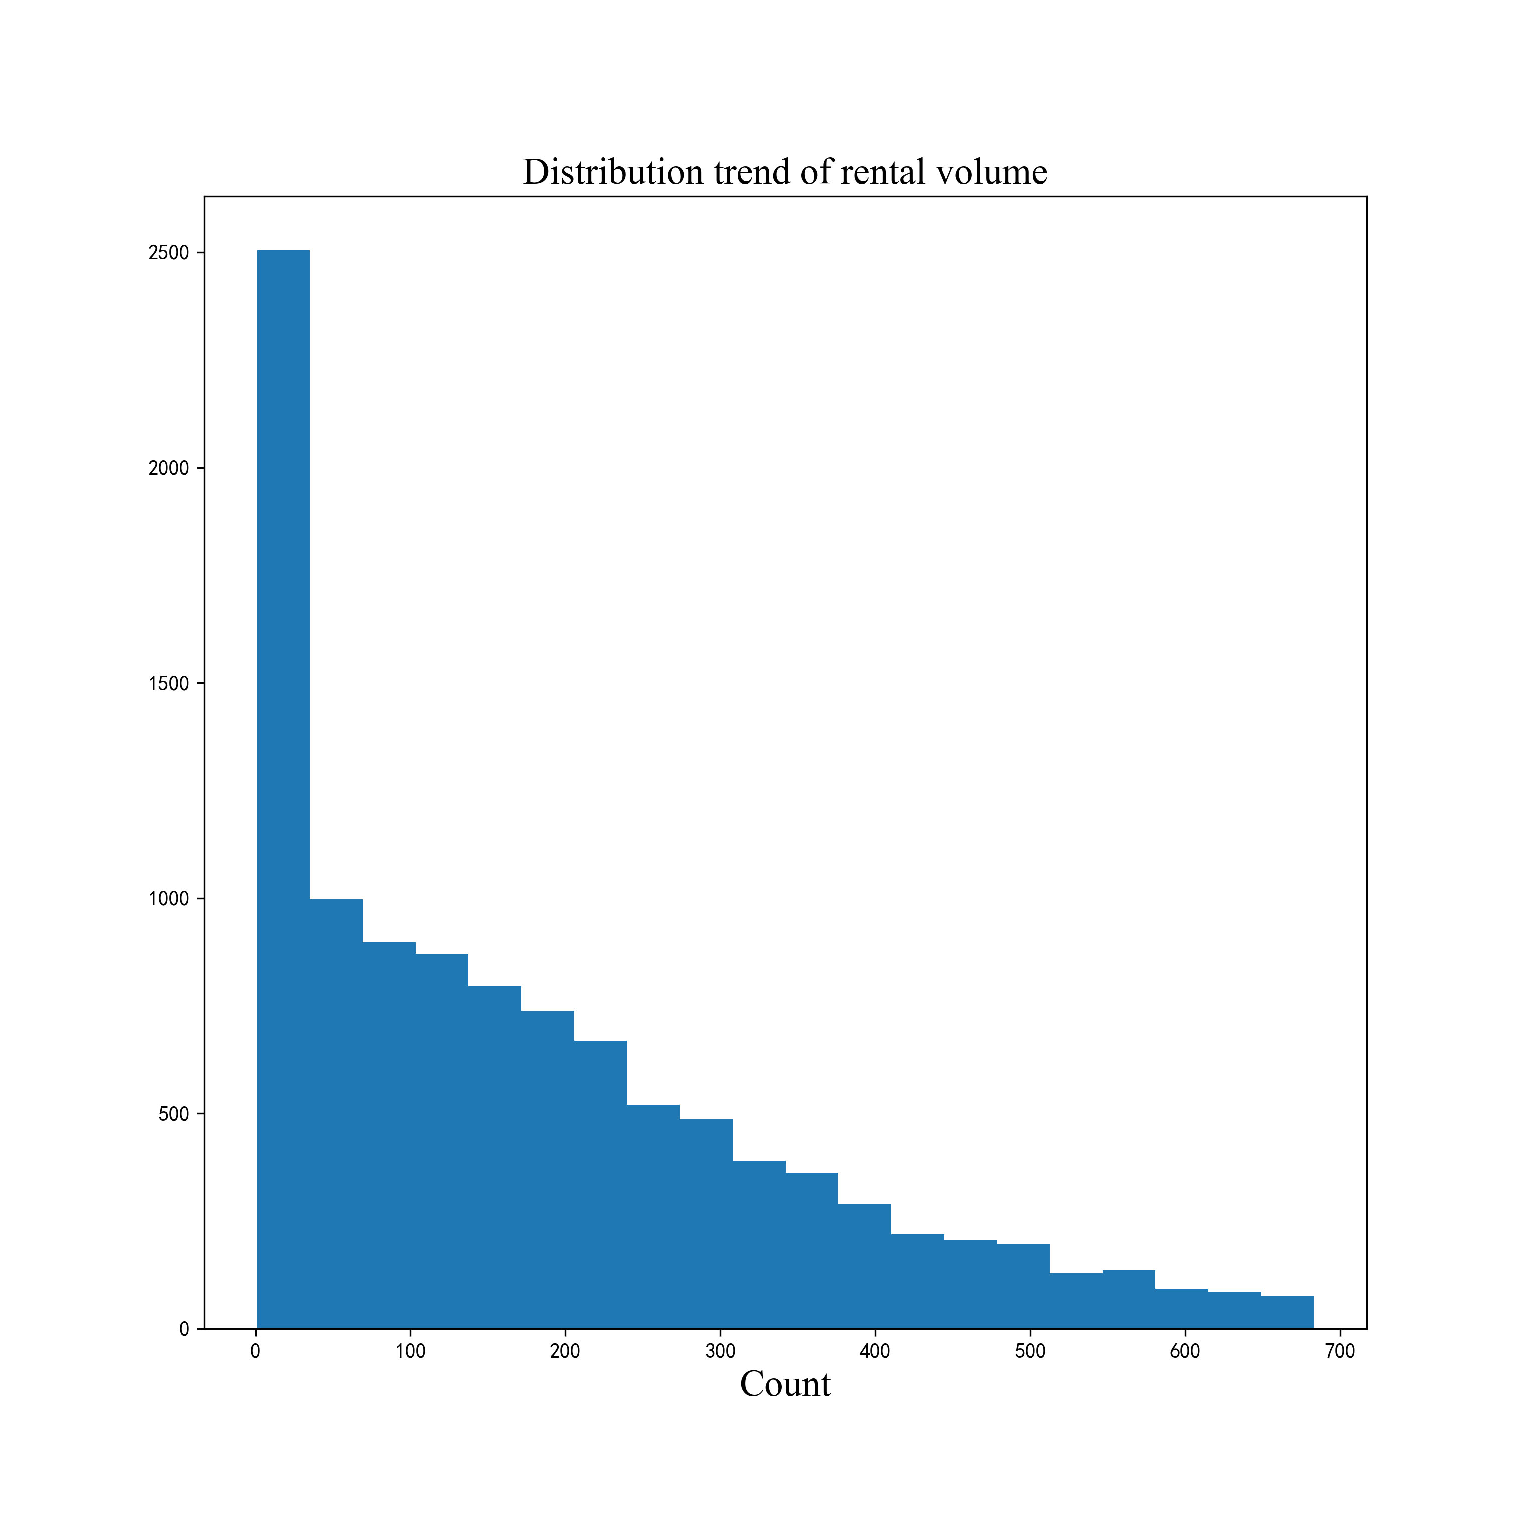
\includegraphics[width=0.5\textwidth]{figures//counts.eps}
          
          %\caption{GOAM Algorithm}\label{OS-Identification}
    
        \end{figure}
       
      \end{slide}



    

      \begin{slide}{Data processing 2}
        % \begin{itemize}
        % \item
        % The whole distribution inclines seriously and needs to be dealt with in order to avoid over fitting in the end.
        % \end{itemize}
        %   \begin{figure}[t]
        %     %\missingfigure[figwidth=16cm]{Testing a long text string}
        %     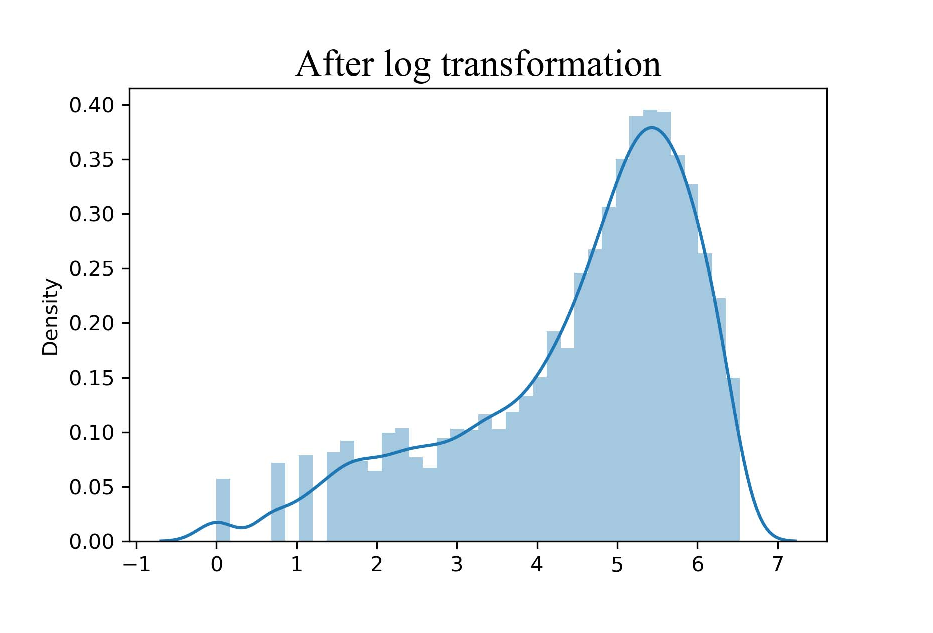
\includegraphics[width=0.5\textwidth]{figures//log.eps}
        %     %\setlength{\belowcaptionskip}{-20pt}\centering\caption{Data processing}
        %     \vspace{-2em}
        %     \caption{Data processing}\label{OS-Identification}
        %   \end{figure}
        \begin{figure}[htbp]
          \centering
          \begin{minipage}[t]{0.48\textwidth}
          \centering
          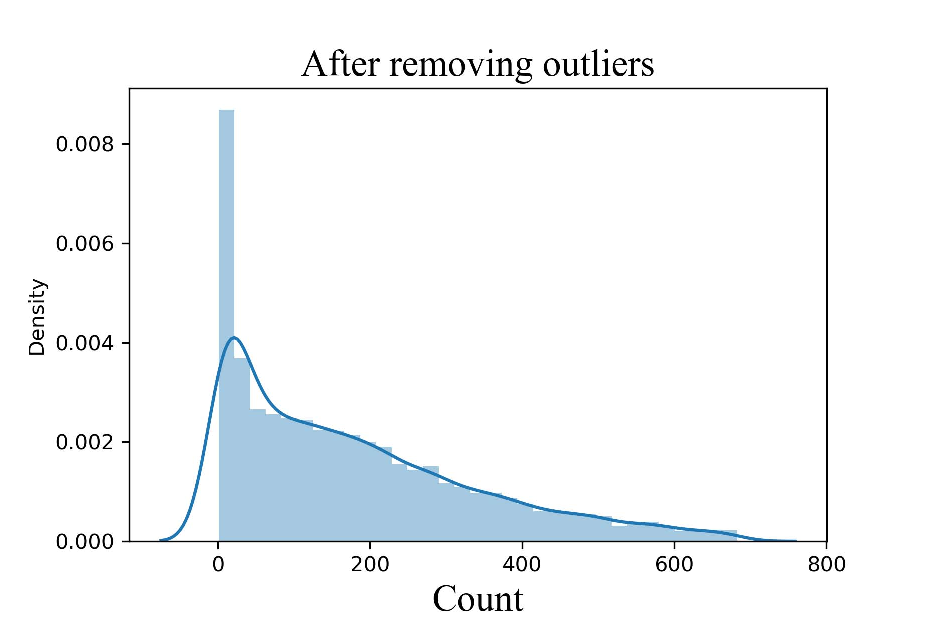
\includegraphics[width=0.9\textwidth]{figures//1_after.eps}
          \vspace{-1.4em}
          \caption{Before treatment}
          \end{minipage}
          \begin{minipage}[t]{0.48\textwidth}
          \centering
          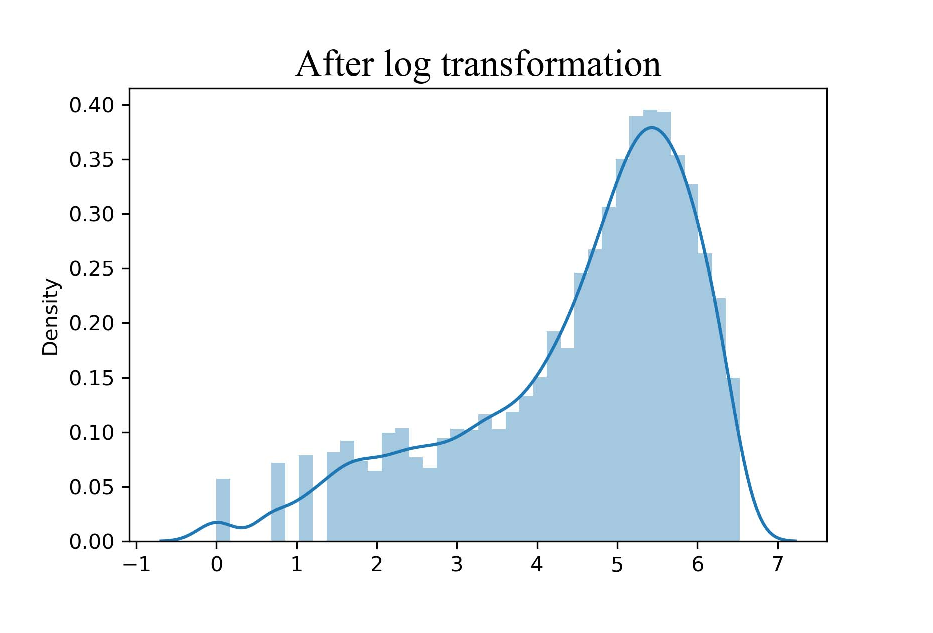
\includegraphics[width=0.9\textwidth]{figures//log.eps}
          \vspace{-1.4em}
          \caption{After treatment}
          \end{minipage}
          \end{figure}
          \begin{itemize}
            \item
            After the conversion, the distribution of the graph is not so severely inclined, and the difference is also smaller.
      
            \end{itemize}
        \end{slide}

        \begin{slide}{Data processing 3}
          
            \begin{figure}[htb]
              \centering
              %\missingfigure[figwidth=16cm]{Testing a long text string}
              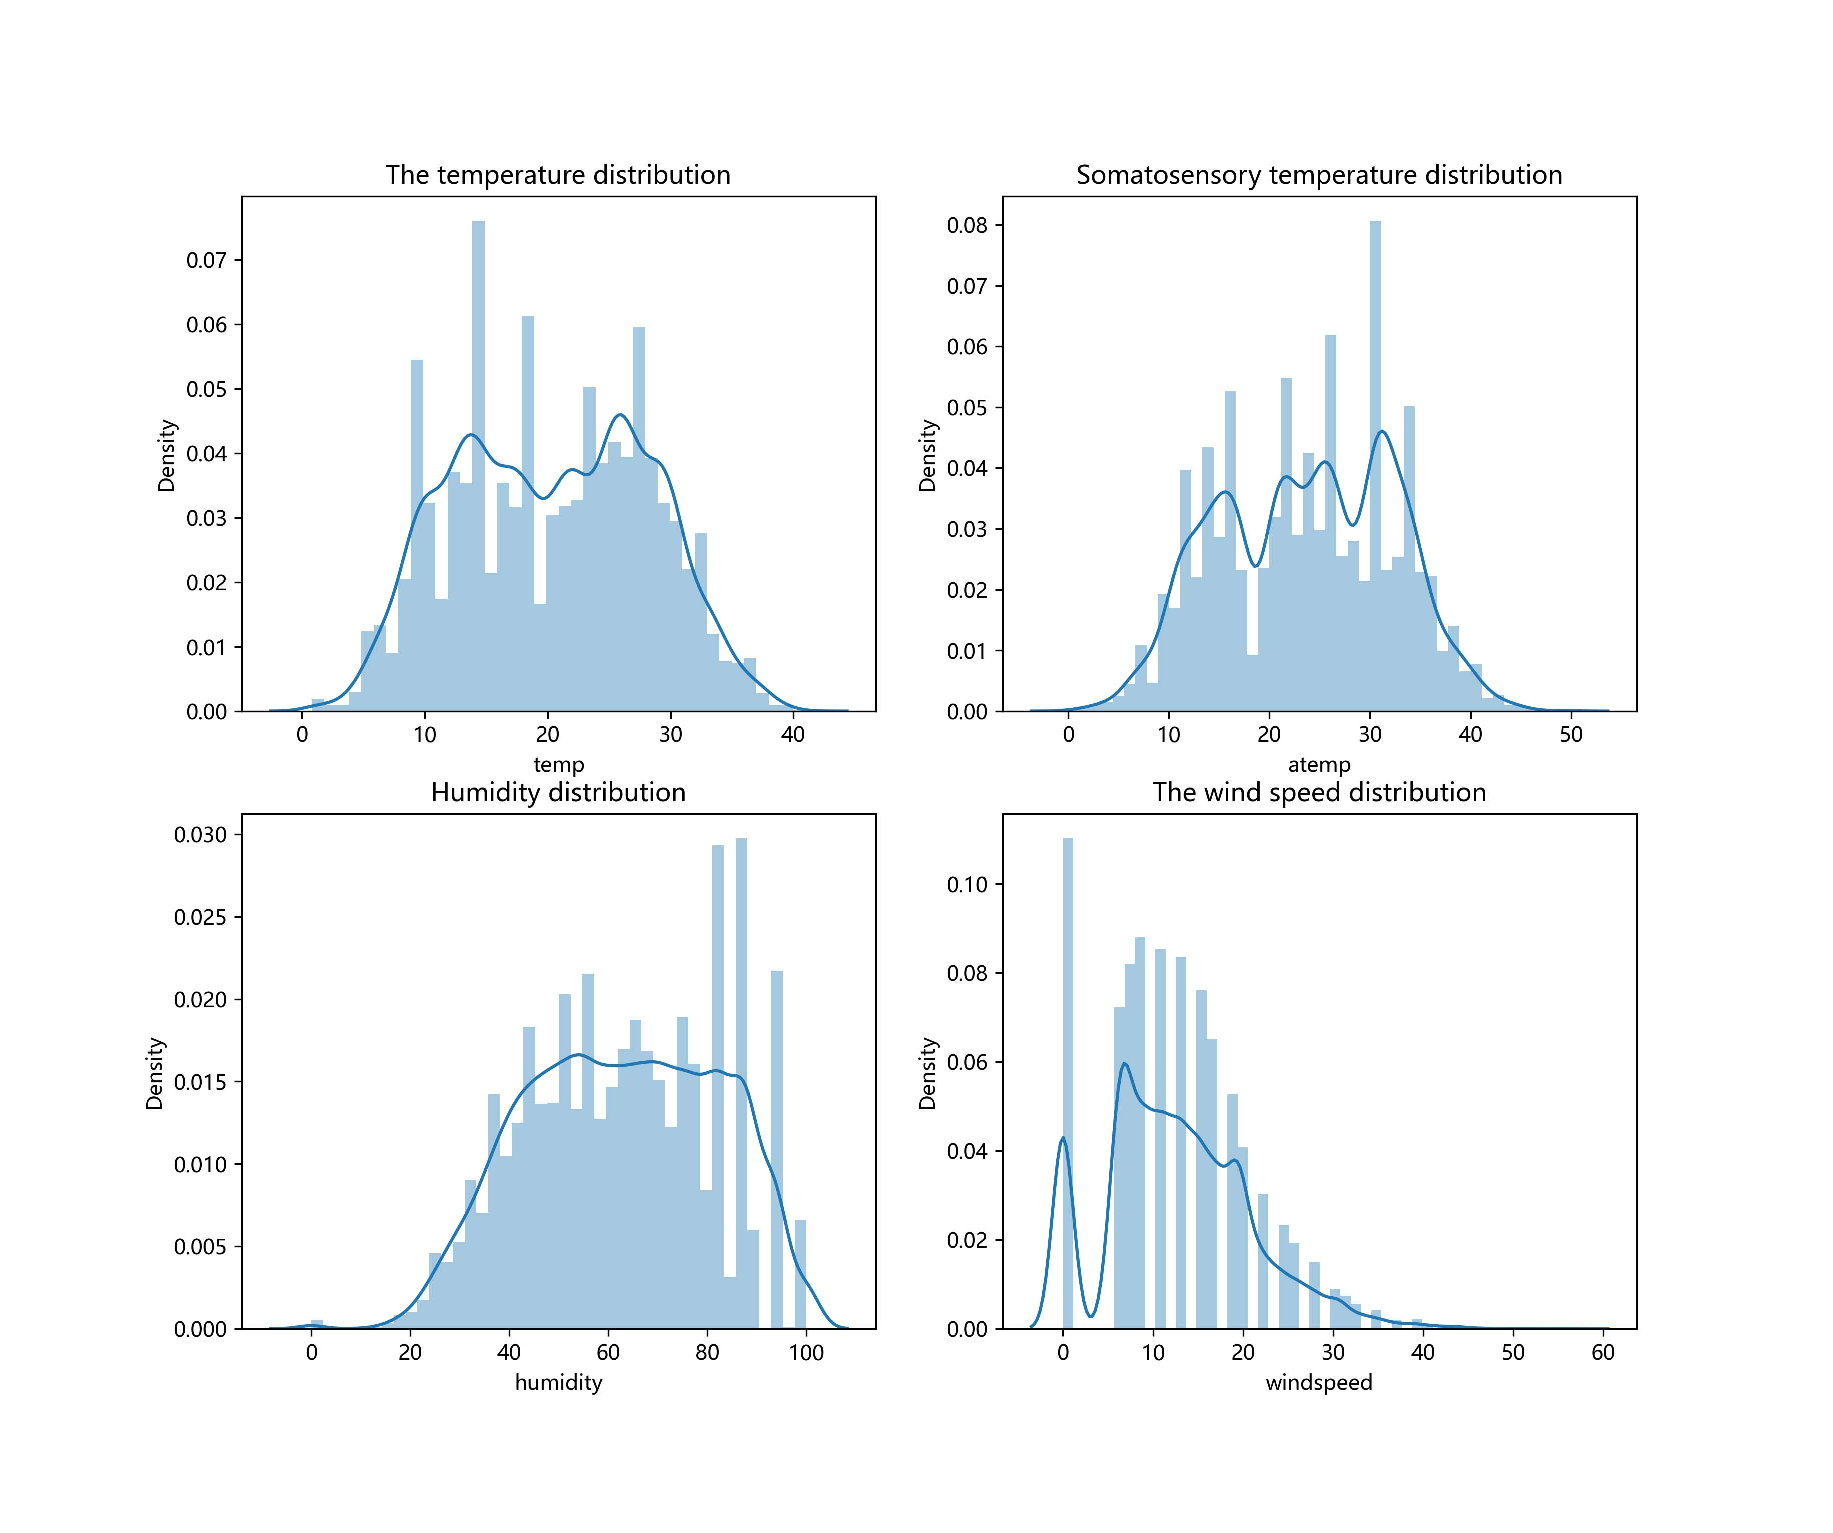
\includegraphics[width=0.6\textwidth,trim=60 60 60 60,clip]{figures//anlysis.eps}
              \vspace{-1.3em}
              \caption{Abnormal data}
            \end{figure}
            %\includegraphics[width=0.5\textwidth,trim=50 50 50 50,clip]{figures/logo.pdf}
            %在此示例中,width制定了图片的缩放比例,trim指定了需要在上下左右裁去的图片宽度,clip表示不显示采取的图片。
            \vspace{-1.4em}
            \begin{itemize}
              \item
              There are some gaps between wind speed 1-6. It is speculated that some wind speed data is missing, but the missing wind speed is filled with 0 in the data.
              \end{itemize}
           
          \end{slide}

          
        \begin{slide}{Data processing 4}
          
          \begin{figure}[htb]
            \centering
            %\missingfigure[figwidth=16cm]{Testing a long text string}
            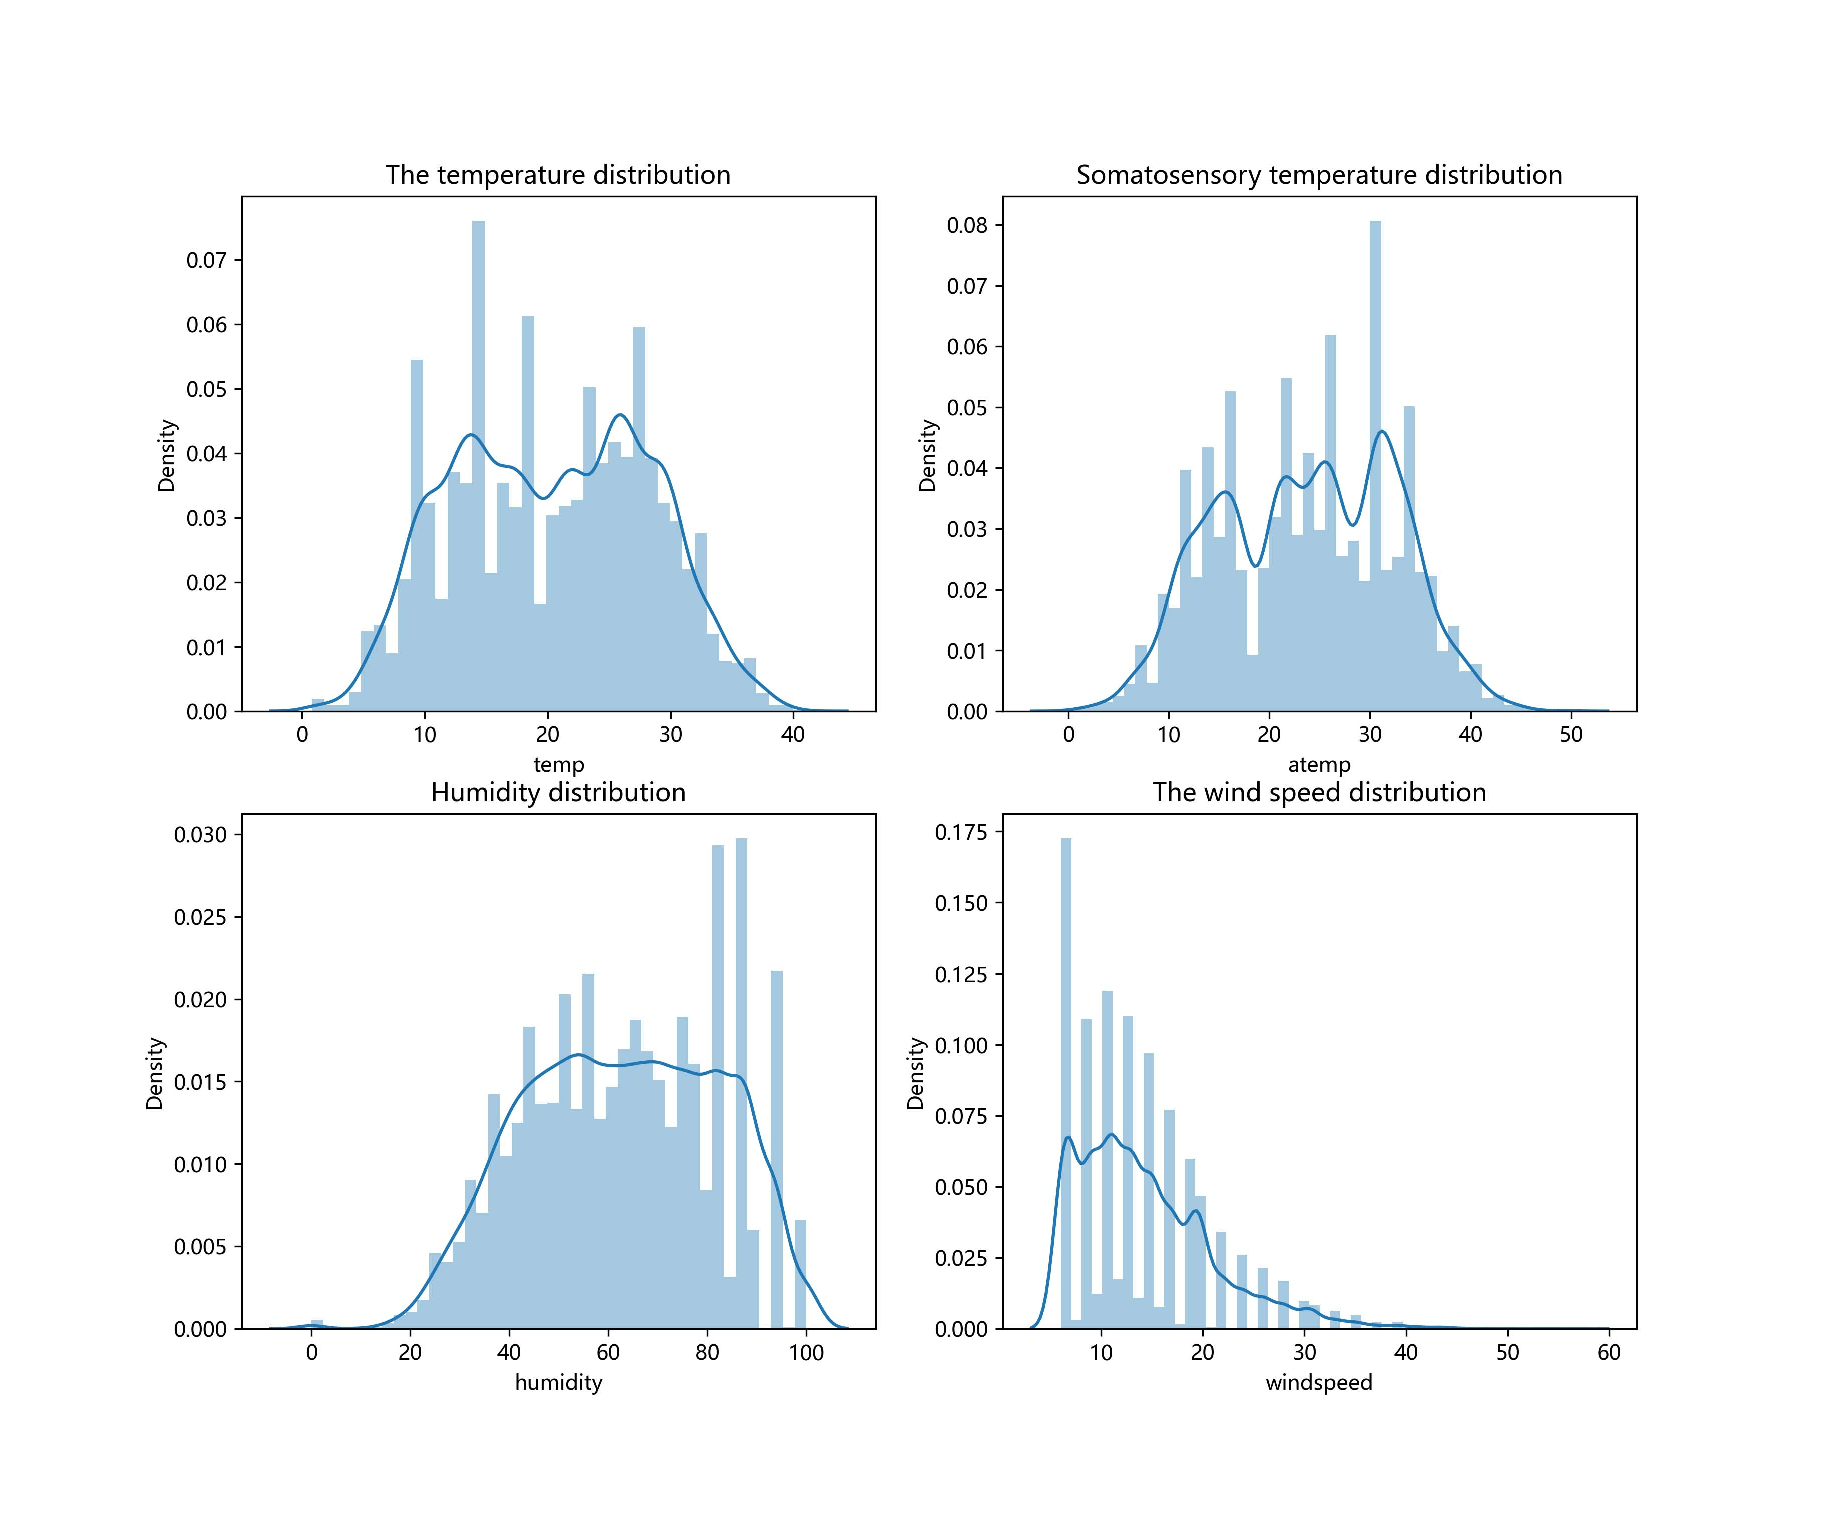
\includegraphics[width=0.6\textwidth,trim=60 60 60 60,clip]{figures//analysis2.eps}
            \vspace{-1.3em}
            \caption{Processed data}
          \end{figure}
          %\includegraphics[width=0.5\textwidth,trim=50 50 50 50,clip]{figures/logo.pdf}
          %在此示例中,width制定了图片的缩放比例,trim指定了需要在上下左右裁去的图片宽度,clip表示不显示采取的图片。
          \vspace{-1.4em}
          \begin{itemize}
            \item
            It can be seen that the feature distribution after filling is relatively normal.
            \end{itemize}
         
        \end{slide}

        \section{Data visualization}   
        \begin{slide}{Data visualization 1}
          
          \begin{figure}[htb]
            \centering
            %\missingfigure[figwidth=16cm]{Testing a long text string}
            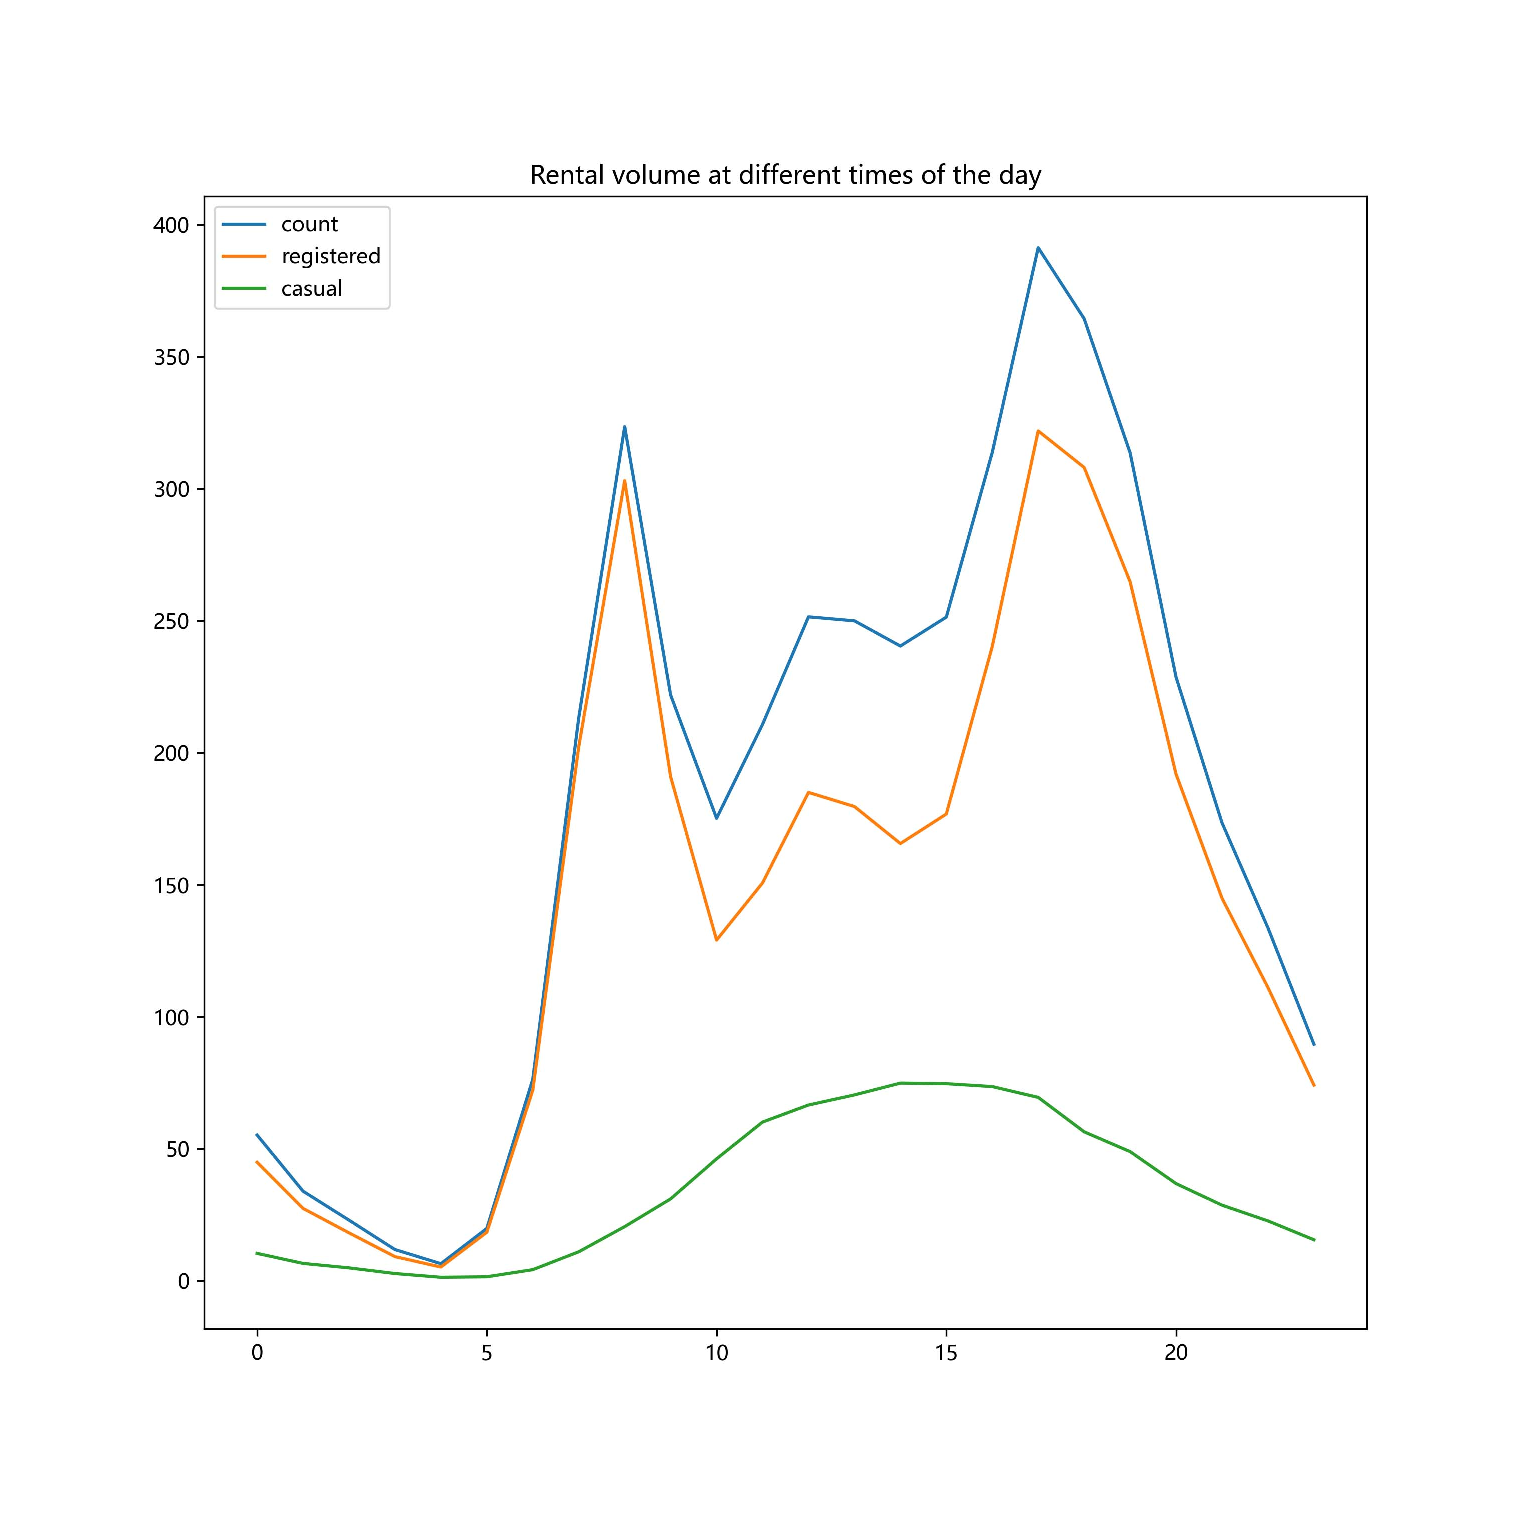
\includegraphics[width=12cm,height=8cm,trim=60 60 60 60,clip]{figures//time_day.eps}
            \vspace{-1.6em}
            \caption{Effect picture}
          \end{figure}
          %\includegraphics[width=0.5\textwidth,trim=50 50 50 50,clip]{figures/logo.pdf}
          %在此示例中,width制定了图片的缩放比例,trim指定了需要在上下左右裁去的图片宽度,clip表示不显示采取的图片。
          \vspace{-1.6em}
          \begin{itemize}
            \item
            7-8 o'clock in the morning, 5-6 o'clock in the afternoon, respectively, the morning peak and evening peak, in line with the actual situation.
            \end{itemize}       
        \end{slide}

        \begin{slide}{Data visualization 2}
          
          \begin{figure}[htb]
            \centering
            %\missingfigure[figwidth=16cm]{Testing a long text string}
            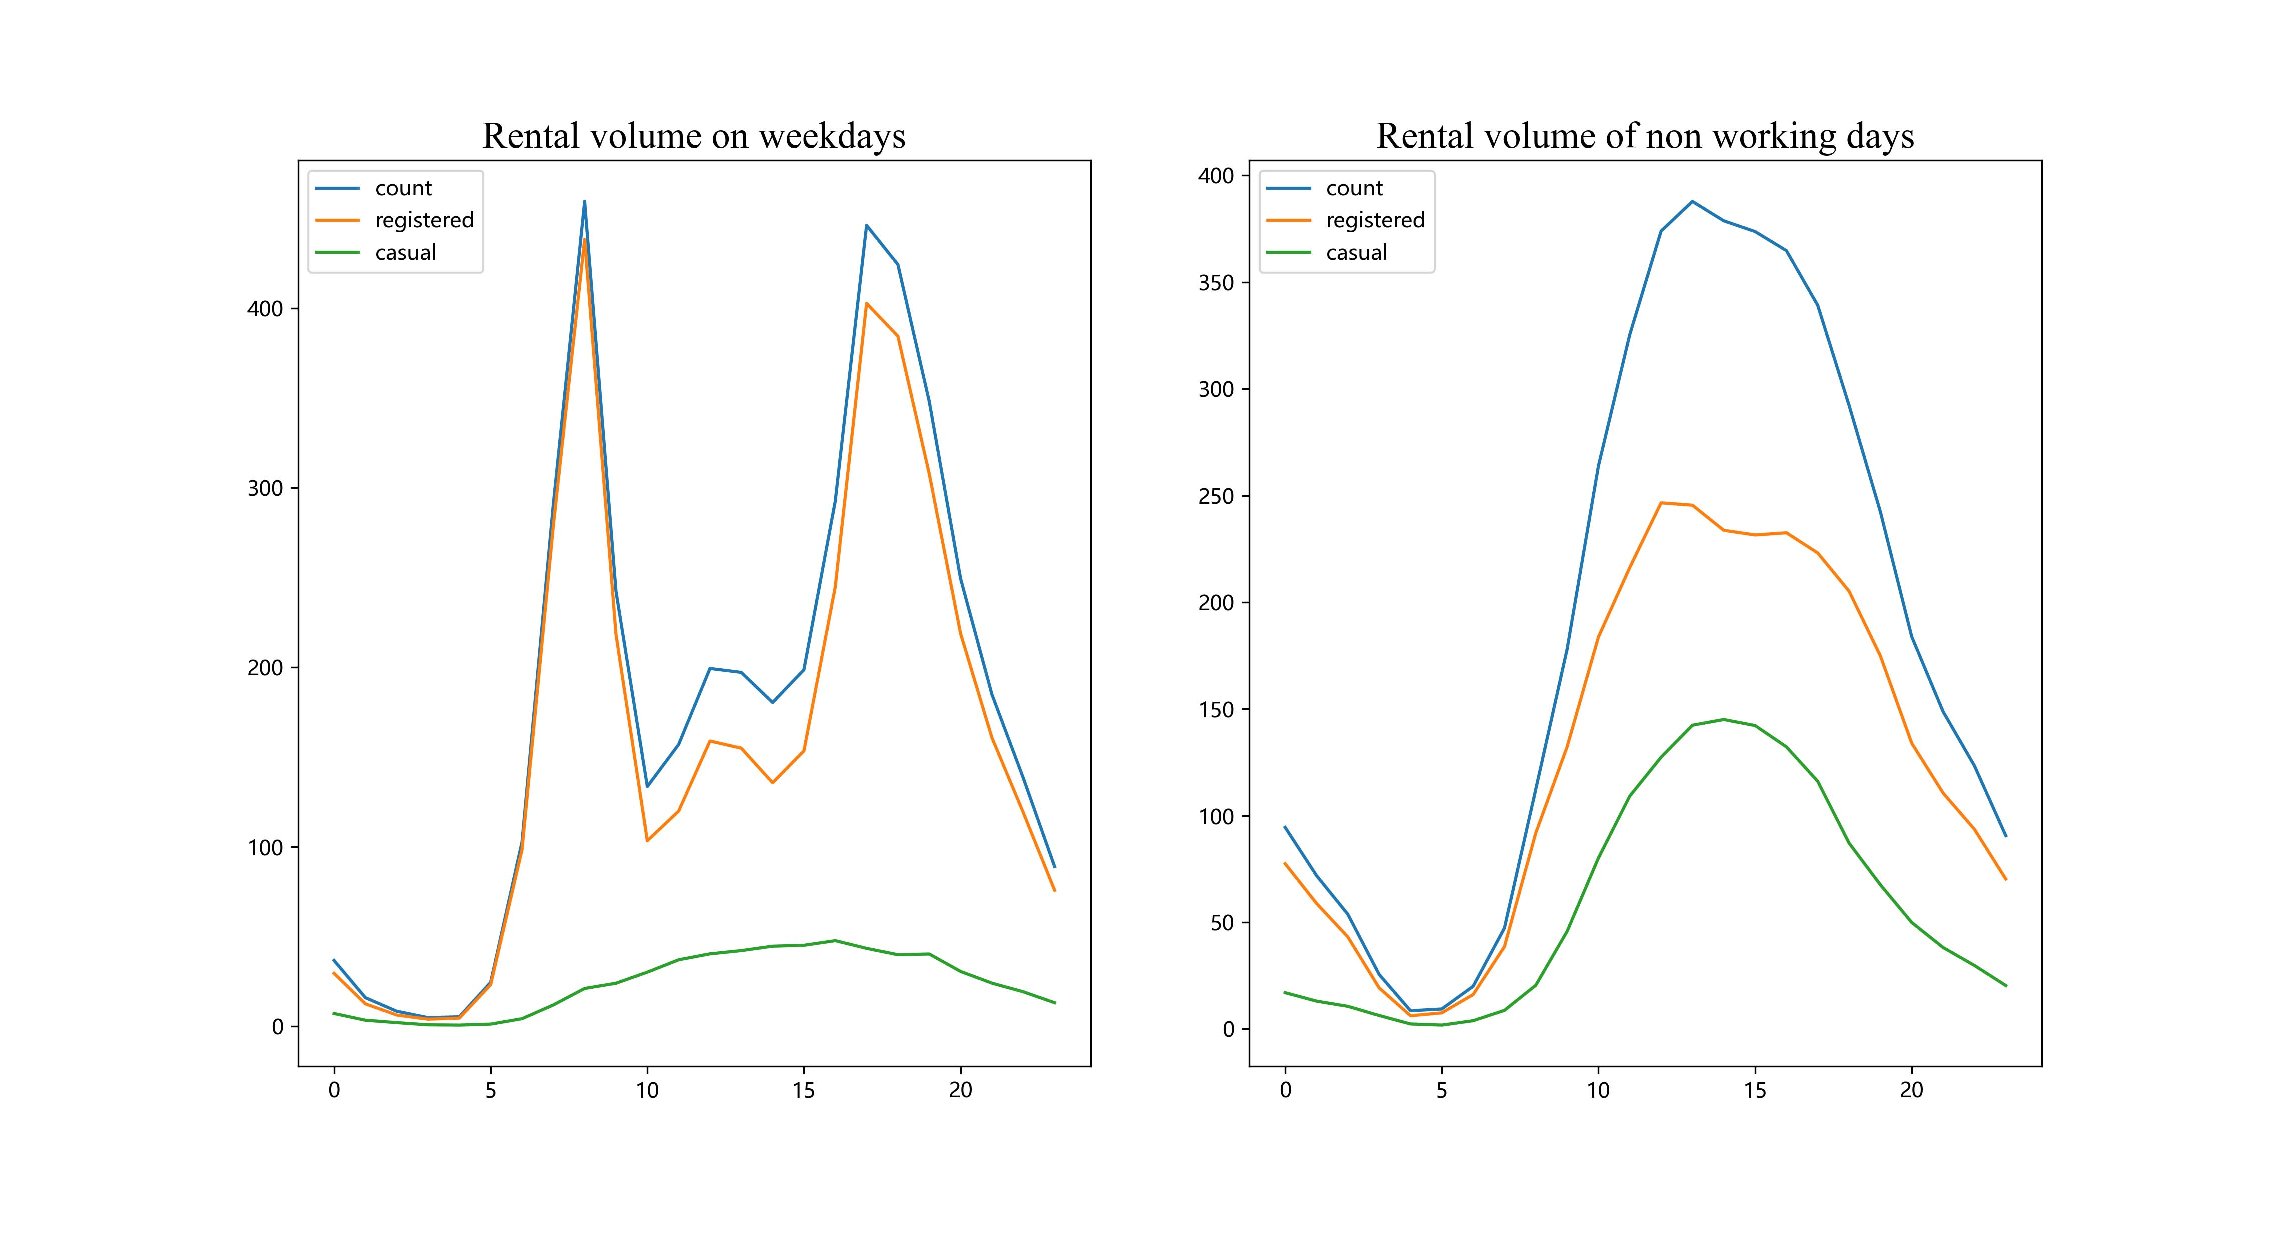
\includegraphics[width=18cm,height=8cm,trim=45 45 45 45,clip]{figures//work-time.eps}
            \vspace{-1.6em}
            \caption{Effect picture}
          \end{figure}
          %\includegraphics[width=0.5\textwidth,trim=50 50 50 50,clip]{figures/logo.pdf}
          %在此示例中,width制定了图片的缩放比例,trim指定了需要在上下左右裁去的图片宽度,clip表示不显示采取的图片。
          \vspace{-1.6em}
          \begin{itemize}
            \item
            By comparing the trend of weekdays and non weekdays, we find that the peak time of commuting is obvious on weekdays, while on non weekdays, people prefer to go out after 2-3 PM.
            \end{itemize}
         
        \end{slide}
   


%%
%%==========================================================================================

% \begin{slide}{Introduction}
% \begin{center}
% \twotonebox{\rotatebox{90}{Defn}}{\parbox{.86\textwidth}
% {Outlying Aspects Mining aims to
% identify the outstanding features of the query object.
% \begin{itemize}
% \item A teacher may be interested in the \textcolor{orange}{characteristics} that
% make \textcolor{orange}{one student} \textcolor{orange}{distinctive} from others.

% find out the strengths and weaknesses of the player (a query object).
% \end{itemize}
% }}
% \end{center}
% \bigskip
% \begin{center}
% \begin{tabular}{c| c c c c }
% \toprule
% Player & \texttt{3PT\%}  & \texttt{FTA} & \texttt{FT\%} & \texttt{To} \\
% \midrule
% $P_1$
% &  {$65$} &  {$4$} &  {$33$} &  {$8$} \\
% $P_2$
% &  {$78$} &  {$1$}&  {$65$}&  {$5$} \\
% $P_3$
% &  {$58$} &  {$6$} &  {$46$} &  {$3$} \\
% $P_4$
% &  {$68$} &  {$1.2$}&  {$85$}&  {$6.2$} \\
% $P_5$
% &  {$58$} &  {$6.2$} &  {$36$} &  {$3.4$}\\
% \bottomrule
% \end{tabular}
% \end{center}
% \bigskip
% \end{slide}

%%==========================================================================================
%----留下

%----留下


%%==========================================================================================
%%

%-----留下来---
\begin{slide}[toc=,bm=]{Data visualization 3}
\begin{itemize}
\item
Come to the conclusion

\begin{itemize}
\item
\smallskip
During the week, Saturdays have the highest rental volume.
\item
\smallskip
Presumably, this is the day when people spend the most time and enjoy going out, and the number of non-registered users is also the highest.
\end{itemize}
\end{itemize}
\vspace{-2.5em}
\begin{figure}[htb]
  \centering
  %\missingfigure[figwidth=16cm]{Testing a long text string}
  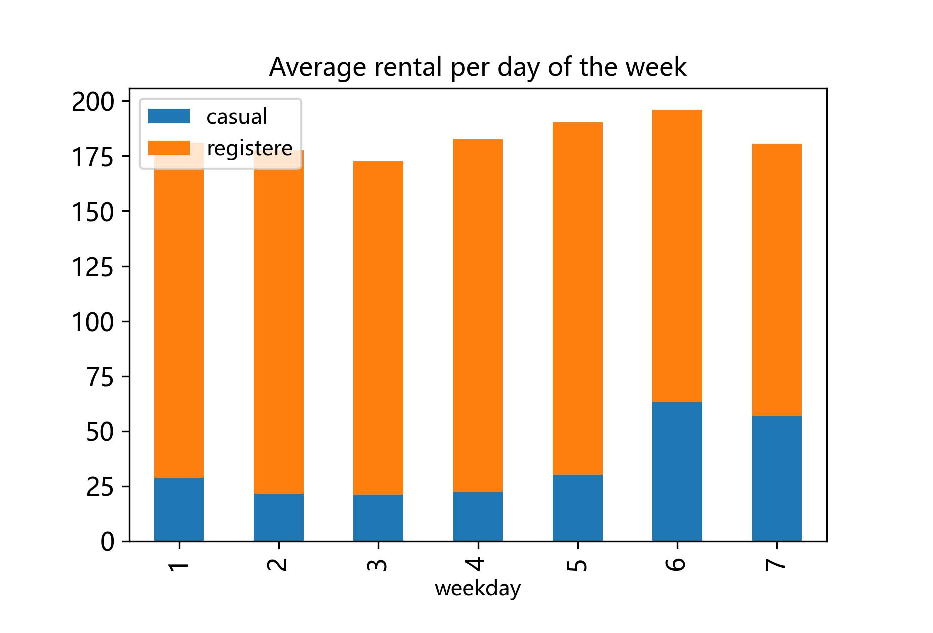
\includegraphics[width=0.62\textwidth]{figures//week-count.eps}
  \vspace{-1.4em}
  \caption{Effect picture}
\end{figure}

\end{slide}
%%
%%==========================================================================================


% \section{Related Work and Challenges}

%---留----
% \begin{slide}[toc=,bm=]{Related Work - Outlying Aspects Mining}

% \begin{itemize}
% \item
% Existing Methods - \textcolor{orange} {Score-and-search}

% \begin{itemize}
% \item
% Define an outlying score function.

% \item
% Search subspaces.
% \end{itemize}
% \bigskip
% \twocolumn[
% \savevalue{lfrheight}=5cm,
% \savevalue{lfrprop}={
% linestyle=solid,framearc=.2,linewidth=1pt},
% rfrheight=\usevalue{lfrheight},
% rfrprop=\usevalue{lfrprop}
% ]{
% Disadvantages
% \begin{itemize}
% \item
% \smallskip
% Dimensionality bias.

% \item
% \smallskip
% Search efficiency is \textcolor{orange}{Not} high (dataset is large).

% \item
% \smallskip
% \textcolor{orange}{Not} identify group outlying aspects.
% \end{itemize}
% }{
% Advantages
% \begin{itemize}
% \item
% \smallskip
% Quantify the outlying degree correctly.

% \item
% \smallskip
% High Comprehensibility.

% \end{itemize}
% }
% \end{itemize}

% \end{slide}
%%
%%==========================================================================================



%%==========================================================================================
%%---留----
\section{The next stage of work}
\begin{slide}{Work}
%Step Three - Outlying Aspects Identification
\begin{itemize}
  \item
  Analyze the influence of weather factors on rental volume.
  \vspace{0.8em}
  \item
  Feature processing and selection.
  \begin{itemize}
  \item
  \smallskip
  The correlation analysis of each factor to the rental volume.
  \end{itemize}
\end{itemize}
  \begin{itemize}
  \item
  Build and evaluate models.
  \begin{itemize}
    \item
    \smallskip
    Create training subsets and test subsets.
    \item
    \smallskip
    Select the optimal parameter.
    \end{itemize}
  \end{itemize}
  \begin{itemize}
    \item
    Generate predictions for bike rentals.
  \end{itemize}
  

\end{slide}
%%

%%==========================================================================================


%%==========================================================================================
%%

%%


% \section{Evaluation Results}




%%==========================================================================================
%%---留---
% \begin{slide}{Synthetic Dataset}

% \begin{itemize}
% \item Synthetic Dataset and Ground Truth
% \end{itemize}

% \begin{table}
% \setlength{\abovecaptionskip}{0pt}
% \setlength{\belowcaptionskip}{10pt}
% \centering
% \caption{Synthetic Dataset and Ground Truth}

% \begin{tabular}{p{2.8cm}p{0.9cm}p{0.9cm}p{0.9cm}p{0.9cm}p{0.9cm}p{0.9cm}p{0.9cm}p{0.9cm}}
% \hline
%   % after \\: \hline or \cline{col1-col2} \cline{col3-col4} ...
%   Query group  & $\mathbf{F_1}$ & $\mathbf{F_2}$ & $F_3$ & $\mathbf{F_4}$ & $F_5$ & $F_6$ & $F_7$ & $F_8$\\
% \hline
%   $i_1$   & \bf{10} & \bf{8}  & 9  & \bf{7}  & 7 & 6 & 6  & 8\\
%   $i_2$   & \bf{9}  & \bf{9}  & 7  & \bf{8}  & 9 & 9 & 8  & 9\\
%   $i_3$   & \bf{8}  & \bf{10} & 8  & \bf{9}  & 6 & 8 & 7  & 8\\
%   $i_4$   & \bf{8}  & \bf{8}  & 6  & \bf{7}  & 8 & 8 & 6  & 7\\
%   $i_5$   & \bf{9}  & \bf{9}  & 9  & \bf{7}  & 7 & 7 & 8  & 8\\
%   $i_6$   & \bf{8}  & \bf{10} & 8  & \bf{8}  & 6 & 6 & 8  & 7\\
%   $i_7$   & \bf{9}  & \bf{9}  & 7  & \bf{9}  & 8 & 8 & 8  & 7\\
%   $i_8$   & \bf{10} & \bf{9}  & 10 & \bf{7}  & 7 & 7 & 7  & 7\\
%   $i_9$   & \bf{9}  & \bf{10} & 8  & \bf{8}  & 7 & 6 & 7  & 7\\
%   $i_{10}$& \bf{9}  & \bf{9}  & 7  & \bf{7}  & 7 & 8 & 8  & 8\\
% \hline
% \end{tabular}
% \end{table}

% \end{slide}

%%



% \begin{slide}[toc=,bm=]{Questions?}
% \begin{center}
% \begin{figure}
%     \animategraphics[autoplay, loop, height=0.4\textheight]{5}{figures//gif//question//q_}{1}{30}
% \end{figure}
% \end{center}
% \end{slide}

\end{document}

\endinput
